
\section{Experimentation}
\label{sec:experimentation}

This section aims at highlighting the properties of \NAME that enables
adaptive scoped broadcast in dynamic networks. Most importantly, it
aims at answering the following questions: Does \NAME allows the
system to reach consistent partitioning? Does \NAME scales well in
large networks? Does \NAME improves scoped broadcast in
inter-autonomous systems? \TODO{Rework this.} We performed the
experimentation using PeerSim, a simulator written in Java that allows
researchers to evaluate and assess distributed algorithms in large
scale networks~\cite{montresor2009peersim}. The code is available on
the Github platform at
\url{https://github.com/Chat-Wane/peersim-partition}.\TODO{Anonoymous.}

\subsection{Confirm the complexity analysis stating that
  communication and time overheads depend on the current partitioning
  of the system.}

\begin{asparadesc}
\item [Description:] We build a network comprising 10k
  processes. First, we chain processes together, then we add another
  communication link per process to another process. Since links are
  bidirectional, each process has 4 communication links on average. We
  set the latency of links between 20 and 40 ms at random following a
  uniform distribution. We set the weight of links between 5 and 15 at
  random following a uniform distribution. Weights and latency are
  different, hence the first $\alpha$ received by a process may not be
  that of its shortest path. It implies more concurrent operations,
  hence more traffic to reach consistent partitioning.

\noindent We evaluate dynamic scoped broadcast. First, we create 100
partitions one at a time: before adding a new partition, consistent
partitioning must be reached. Second, we remove every partition one at
a time, in the order of their creation, hence starting from the first
and oldest partition that had been added.

\noindent We focus on the complexity of \NAME. We measure the average
number of messages generated per process during the experiment; and
the time before reaching consistent partitioning after adding or
removing a partition.

\begin{figure}
  \centering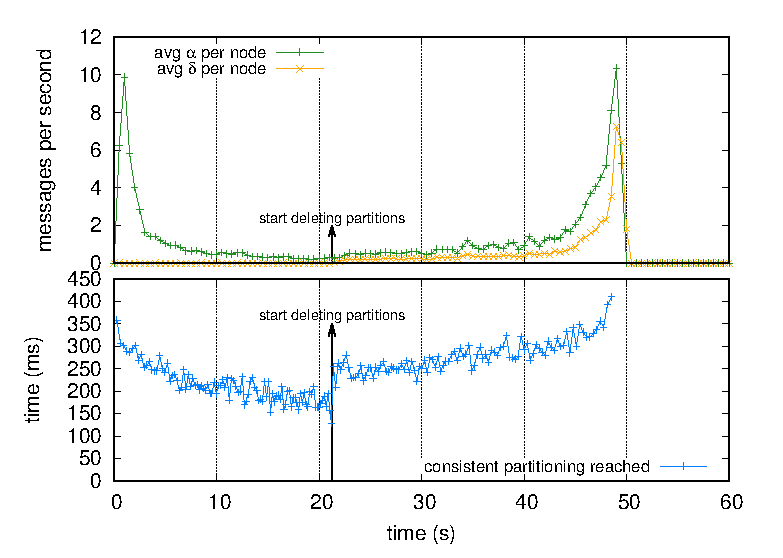
\includegraphics[width=0.99\columnwidth]{img/as_cast_complexity.eps}
  \caption{\label{fig:complexity}Overhead of, and time before,
    reaching consistent partitioning using \NAME.}
  %% \caption{\label{fig:complexity}Cumulative average number of messages
  %%   per process in a network comprising 10k processes; along with the
  %%   duration before reaching consistent partitioning after adding or
  %%   removing a partition, totaling 100 new partition then removed.}
\end{figure}

\item [Results:]

Figure~\ref{fig:complexity} shows the results of this experiment. The
top part of the figure shows the average traffic per process divided
between $\alpha$ and $\delta$ messages. The bottom part of the figure
shows the time before reaching consistent partitioning.

\noindent Figure~\ref{fig:complexity} confirms that \NAME's overhead
depends on the size of partitions. The first partition is the most
expensive, for $\alpha$'s must reach every process which takes time
and generate more traffic. Still, being reactive, as opposed as
cycle-based protocols~\cite{jelasity2007gossip}, \NAME quickly
converge towards consistent partitioning in only 350 milliseconds. The
last and $100^{th}$ partition added around 21 seconds is the least
expensive. By using scoped broadcast, control information only reaches
a small subset of the whole network.

\noindent Figure~\ref{fig:complexity} also confirms that \NAME's
delete operations are more expensive than add operations. Indeed, the
top part of the figure shows that after 21 seconds, when the
experiment involves removals, traffic includes both $\alpha$'s and
$\delta$'s. The latter aims at removing stale information and
triggering competition while the former aims at updating shortest
paths. As corollary, the convergence time increases, for $\delta$'s
must reach every partition border before any sound competitors
propagate their partition. It is worth noting that this delete
operation involves concurrency: removals continue to propagate while
the competition is already partially triggered and propagating.

\noindent Figure~\ref{fig:complexity} shows that the overhead of
adding the $1^{st}$ partition does not correspond to the overhead of
deleting this $1^{st}$ partition. When adding it, messages must reach
all processes while when removing it, messages must reach a small
subset of this membership. This is important, for it means that
\NAME's overhead actually depends on the current partitioning, and
does not depend on the past partitioning.

\noindent Finally, Figure~\ref{fig:complexity} highlights that after
49 seconds, i.e., after the 100 adds and the 100 deletes, processes do
not generate traffic anymore. Being reactive, \NAME has no overhead
when there is no operation in the system. This is important, for it
means that \NAME's overhead actually depends on its usage.

\end{asparadesc}

\subsection{Distribution and hotspots}


\subsection{Inter-autonomous systems}

% \subsection{Use case: caching}
% \subsection{Use case: routing}
% \subsection{Use case: broadcast domain}


%%% Local Variables: 
%%% mode: latex
%%% TeX-master: "../paper"
%%% ispell-local-dictionary: "english"
%%% End: 
